\documentclass[10pt,a4paper]{article}
\usepackage[utf8]{inputenc}
\usepackage[T1]{fontenc}
\IfFileExists{brazil.ldf}{\usepackage[brazil]{babel}}{\renewcommand{\refname}{Referências}}
\usepackage[margin=2cm]{geometry}
\usepackage{booktabs,tabularx,array,graphicx}
\usepackage[hidelinks]{hyperref}
\usepackage[expansion=false]{microtype}
\setlength{\parindent}{0pt}
\setlength{\parskip}{5pt}
\newcolumntype{Y}{>{\raggedright\arraybackslash}X}
\title{AutoML versus meta-aprendizagem\\em regressão desbalanceada}
\author{Carlos Henrique Dias\\\small IN1097 --- Atividade prática 4}
\date{}

\begin{document}
\maketitle
\vspace{-0.5cm}
\begin{center}\small
Código, notebook executado e resultados brutos por dataset e fold:\\
\url{https://github.com/carloshendvpm/projeto01-mtl/tree/entrega-pratica-04/pratica-04}
\end{center}

\section{Objetivo e protocolo}

Na Prática 1, recomendei um regressor para cada dataset a partir de suas meta-características. Na Prática 3, usei datasets parecidos para escolher os pontos iniciais da busca de hiperparâmetros do Random Forest. Os dois métodos dependem de meta-conhecimento construído antes, sobre os mesmos 30 datasets de regressão desbalanceada. Nesta prática, comparei esses métodos com sistemas de AutoML, que buscam o modelo do zero em cada dataset novo, e medi a partir de que orçamento a busca compensa. Como o tema da minha pesquisa é seleção dinâmica para regressão desbalanceada, incluí também a DESReg \cite{desreg}.

O protocolo é o mesmo das práticas anteriores: dez folds com embaralhamento e semente 42. A métrica é a SERA \cite{ribeiro}, que soma os erros quadráticos dos exemplos cuja relevância $\varphi(y)$ passa de um limiar e integra essa soma sobre todos os limiares. Assim, erros nos valores raros do alvo pesam mais. A relevância é estimada automaticamente a partir do alvo do conjunto avaliado.

Cada sistema recebe apenas o treino do fold e faz sua própria validação. O teste é usado uma única vez, para medir a SERA do modelo final. A matriz P das práticas anteriores tem o desempenho de seis regressores com hiperparâmetros padrão: árvore de decisão (DT), gradient boosting (GB), kNN, regressão linear, RF e SVR. Reexecutei esses seis regressores nas mesmas partições. O melhor regressor coincide com o da Prática 1 nos 30 datasets, e a diferença relativa mediana das perdas é $2{,}5\times10^{-7}$.

Não há AutoML voltado para regressão desbalanceada, então escolhi dois sistemas gerais que aceitam métrica customizada e que usam meta-conhecimento de formas diferentes. Ambos otimizam a SERA.

\begin{itemize}
\item \textbf{FLAML 2.8} \cite{flaml}. Busca entre LightGBM, XGBoost, CatBoost, RF, Extra Trees e regressão linear com SGD. A cada passo, escolhe qual estimador testar pelo custo e pela melhora esperada, e ajusta os hiperparâmetros de cada um por uma busca local que começa nas configurações mais baratas (Cost-Frugal Optimization). Rodei o FLAML de duas formas: com os pontos iniciais fixos e com um portfólio zero-shot aprendido em datasets do OpenML (\texttt{starting\_points="data"}), que chamo de FLAML+zs. Esse portfólio usa as características do treino para definir a ordem dos estimadores e os pontos de partida. Ele faz ao mesmo tempo o papel da MtL e do warm-start, e desligá-lo permite medir seu efeito.
\item \textbf{AutoGluon 1.6} \cite{autogluon}. No preset \texttt{medium\_quality}, treina uma lista fixa de modelos (GBMs, RF, Extra Trees, kNN e redes neurais). Depois, combina os modelos por seleção gulosa em um conjunto de validação separado. Seu meta-conhecimento é essa lista, igual para todo dataset. Ela se parece mais com o Melhor médio do que com a MtL.
\end{itemize}

Os orçamentos foram de 5, 30 e 120 s por fold, exceto o FLAML sem portfólio, que não rodou a 120 s por falta de tempo. Foram 2.400 execuções, cerca de 24 h de relógio, em um Apple M2 com 8 núcleos e 8 GB, com quatro execuções simultâneas de 2 CPUs cada. O tempo medido nem sempre bate com o orçamento. O AutoGluon para antes do limite nos datasets pequenos. O FLAML+zs passa do limite com frequência: a 5 s, a média foi de 8,8 s.

Também encontrei um erro no FLAML+zs. Em datasets maiores, o portfólio sugere hiperparâmetros que não existem no espaço de busca, e a execução para com \texttt{KeyError}. Alterei a checagem de validade dos pontos iniciais para descartar esses pontos e refiz as 28 execuções que tinham falhado.

Os métodos sem AutoML são estes:

\begin{center}\small
\begin{tabularx}{\linewidth}{lY}
\toprule
Método & Como funciona \\
\midrule
Melhor médio & Regressor de melhor rank médio nos outros 29 datasets (sempre RF), com hiperparâmetros padrão. \\
MtL & Abordagem 2 da Prática 1. Um RF prevê o rank dos seis regressores a partir das 13 meta-características básicas (Xbase), em leave-one-dataset-out. Na Prática 2, a versão estendida não melhorou a recomendação de forma significativa, então mantive a mais barata. Recomenda RF em 22 datasets e GB em 8. \\
Warm-start & Busca bayesiana da Prática 3 em 60 configurações de RF, com 20 avaliações. Começa pelas melhores configurações dos 3 datasets mais próximos em Xestendido, que soma a Xbase medidas de complexidade calculadas no alvo inteiro e, separadamente, nos exemplos comuns e nos raros. \\
DESReg, DESReg-$\varphi$ & Seleção dinâmica sobre 60 modelos (bagging de 10 de cada regressor de P). A competência é o erro local; na segunda versão, ponderado por $1+\varphi(y)$. \\
Oráculo & O melhor dos seis regressores de P em cada dataset, escolhido olhando o teste. Serve só de referência. \\
\bottomrule
\end{tabularx}
\end{center}

O Warm-start foi refeito. Na Prática 3, a busca consultava uma matriz de perdas calculada com os próprios folds de teste. Aqui, cada avaliação usa validação cruzada de 3 folds dentro do treino, como fazem os sistemas de AutoML.

\section{Desempenho}

Como as escalas de SERA variam muito entre datasets, usei a perda relativa: a SERA do método dividida pela menor SERA obtida no dataset, menos 1. Reporto a mediana porque a média é dominada por poucos casos. Em \texttt{heat}, por exemplo, o FLAML sem portfólio chega a SERA 29 e o AutoGluon a 120 s chega a 37, enquanto todos os regressores de P ficam acima de 1.500. O rank médio é calculado entre os 13 métodos; do oráculo, mostro só a perda. Vitórias conta os datasets em que o método teve sozinho a menor SERA; empates não entram. A última coluna é o tempo medido; no Warm-start, inclui a extração de Xestendido.

\begin{center}\small
\begin{tabular}{lrrrr}
\toprule
Método & Rank médio & Perda rel.\ mediana & Vitórias & s por fold \\
\midrule
AutoGluon 120 s & 4,33 & 0,020 & 8 & 65,4 \\
AutoGluon 30 s & 5,03 & 0,123 & 1 & 26,2 \\
Warm-start & 5,90 & 0,279 & 0 & 32,3 \\
FLAML+zs 120 s & 6,47 & 0,159 & 3 & 111,4 \\
Melhor médio & 6,53 & 0,300 & 0 & 1,5 \\
FLAML+zs 30 s & 6,78 & 0,178 & 3 & 32,6 \\
MtL & 6,83 & 0,319 & 0 & 1,3 \\
FLAML+zs 5 s & 7,08 & 0,288 & 1 & 8,8 \\
FLAML 30 s & 7,32 & 0,195 & 1 & 31,0 \\
AutoGluon 5 s & 7,57 & 0,308 & 1 & 8,3 \\
FLAML 5 s & 8,35 & 0,434 & 1 & 5,7 \\
DESReg-$\varphi$ & 9,10 & 0,490 & 1 & 31,8 \\
DESReg & 9,70 & 0,551 & 0 & 31,8 \\
Oráculo &  & 0,198 &  &  \\
\bottomrule
\end{tabular}
\end{center}

Fiz um teste de Friedman para cada orçamento, com os métodos sem AutoML e os AutoML daquele orçamento. Os três testes rejeitam a igualdade ($p=4{,}4\times10^{-5}$, $3{,}0\times10^{-6}$ e $1{,}8\times10^{-6}$). A Figura~\ref{fig:cd} mostra o pós-teste de Nemenyi com $\alpha=0{,}05$.

\begin{figure}[tbp]
\centering
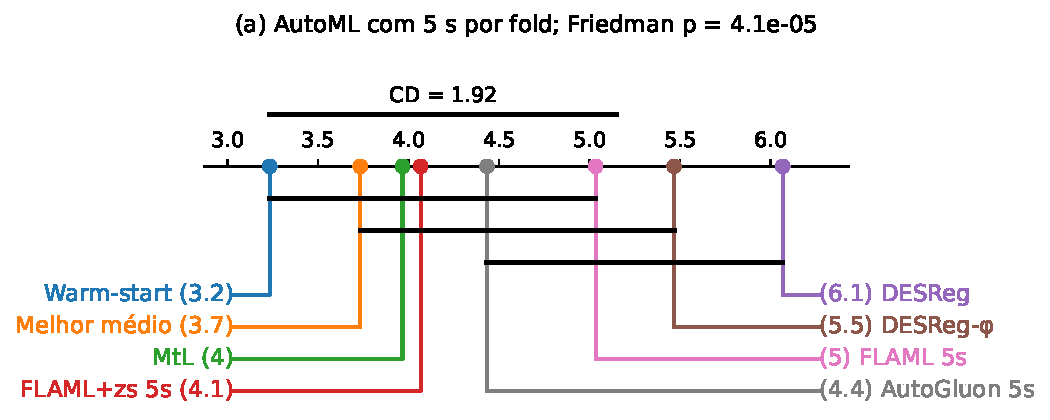
\includegraphics[width=.64\linewidth]{resultados/figuras/cd_5s.pdf}\par
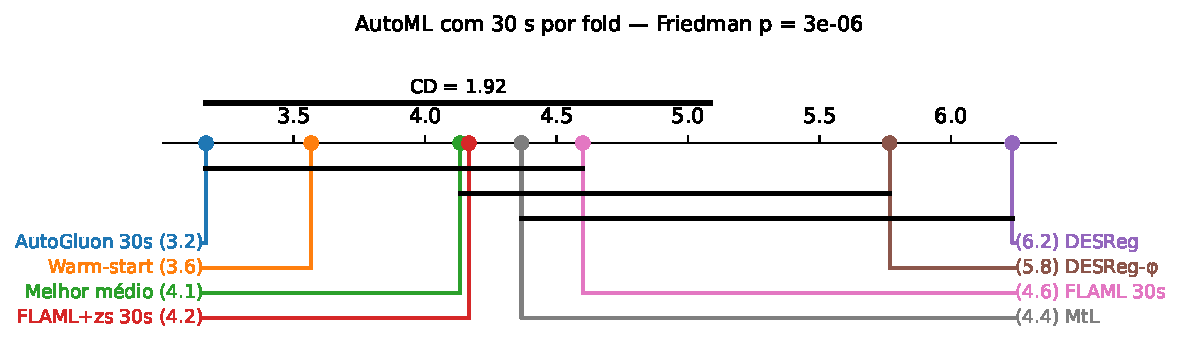
\includegraphics[width=.64\linewidth]{resultados/figuras/cd_30s.pdf}\par
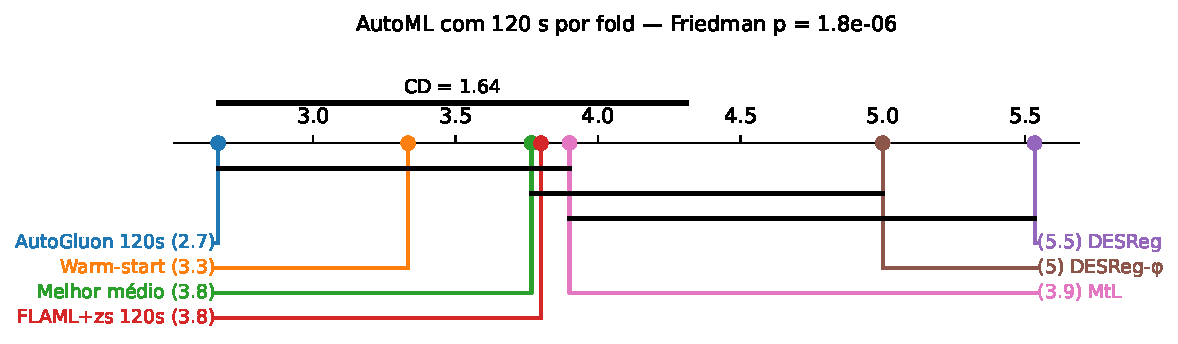
\includegraphics[width=.64\linewidth]{resultados/figuras/cd_120s.pdf}
\caption{Diagramas de diferença crítica (Nemenyi, $\alpha=0{,}05$) por orçamento. Métodos ligados por uma barra não diferem significativamente.}
\label{fig:cd}
\end{figure}

Com 5 s, Warm-start (que leva cerca de 32 s por fold), Melhor médio e MtL ocupam as três primeiras posições. Em rank, nenhum AutoML de 5 s supera um RF padrão, embora o FLAML+zs já tenha SERA menor que a da MtL em 16 datasets. A partir de 30 s, o AutoGluon passa a liderar, com rank 3,2 a 30 s e 2,7 a 120 s. Esses ranks diferem dos da tabela porque cada diagrama compara só 7 ou 8 métodos. Mesmo assim, só as duas DESReg diferem significativamente dele. A 120 s, o AutoGluon tem SERA menor que a da MtL em 20 dos 30 datasets, mas a diferença de rank não é significativa ($p=0{,}29$).

Para separar o que vem de escolher melhor entre os mesmos seis regressores do que vem de usar um espaço maior, comparei a MtL e o AutoGluon a 120 s com o oráculo. A MtL erra o melhor regressor em 18 datasets e fica, em mediana, 3,8\% acima da SERA do oráculo; quase não se afasta do Melhor médio, e só é melhor que ele em 2 datasets. Já o AutoGluon a 120 s fica abaixo da SERA do oráculo em 18 datasets, com ganho mediano de 8\%. Mesmo uma MtL que acertasse sempre ficaria presa ao teto dos seis regressores com hiperparâmetros padrão, e boa parte da vantagem do AutoML vem de sair desse espaço. O Warm-start mostra o mesmo em menor escala: só ajustando os hiperparâmetros do RF, já supera o Melhor médio em 19 datasets.

As duas versões da DESReg ficaram em último lugar nos três orçamentos. Ponderar a competência pela relevância melhora a DESReg em 22 datasets, mas a DESReg-$\varphi$ ainda supera o Melhor médio em apenas 7.

\section{Custo}

O custo online é o tempo por fold para produzir o modelo de um dataset novo. Na MtL, inclui extrair Xbase, consultar o meta-modelo e treinar o regressor. No Warm-start, inclui extrair Xestendido e fazer as 20 avaliações. No AutoML, é a execução inteira. O custo offline é o tempo de CPU gasto para montar o meta-conhecimento: 0,26 h para a MtL (matriz P e Xbase) e 8,8 h para o Warm-start (matriz de perdas da Prática 3 e Xestendido). O portfólio do FLAML e a lista do AutoGluon foram montados pelos autores desses sistemas, e não tenho como medir esse custo.

\begin{center}
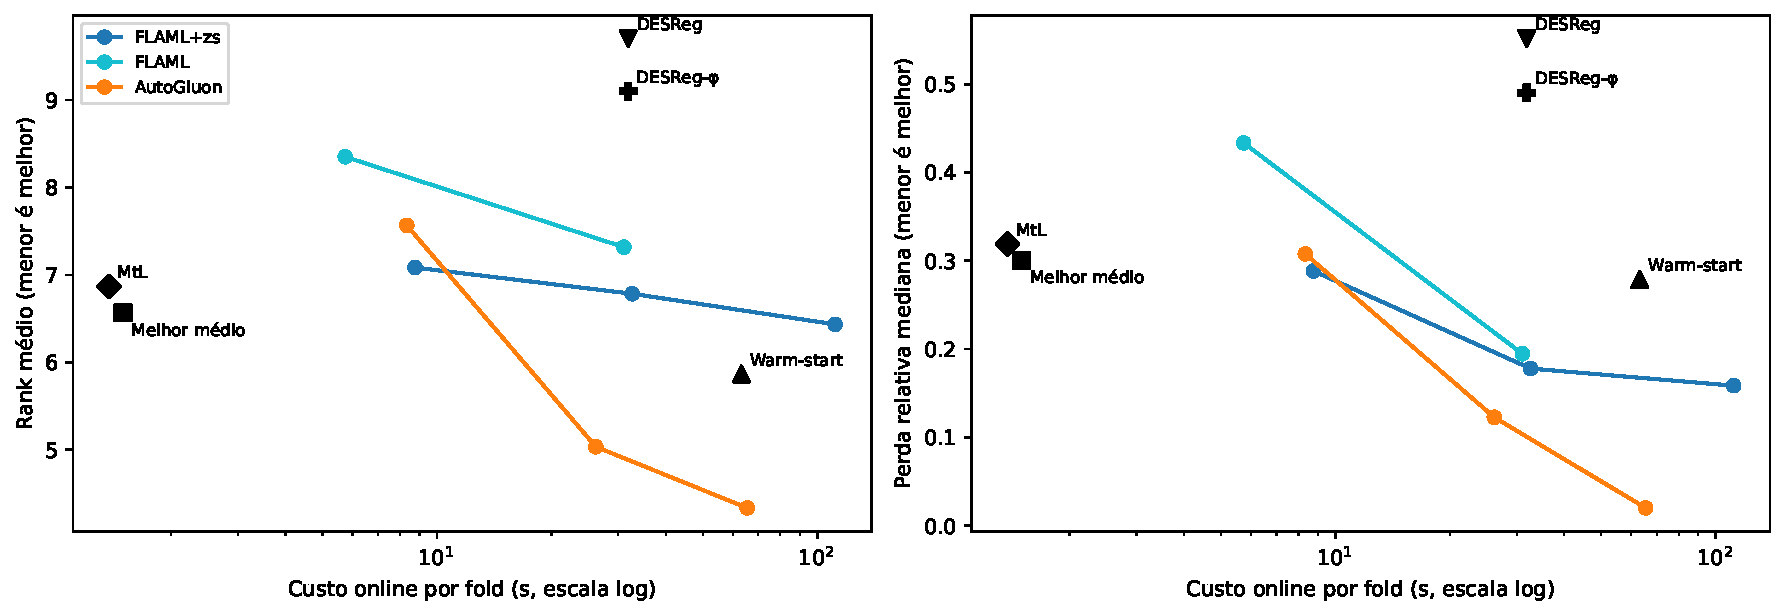
\includegraphics[width=.88\linewidth]{resultados/figuras/custo_desempenho.pdf}
\end{center}

Por fold, a MtL custa 1,3 s, cerca de 50 vezes menos que o AutoGluon a 120 s. Seu rank é melhor que o dos três AutoML de 5 s, e sua perda mediana (0,319) fica entre as deles (0,288 a 0,434). Com 30 s ou mais, o AutoGluon fica à frente tanto em rank quanto em perda mediana. Já o FLAML+zs melhora pouco de 30 para 120 s.

A tabela abaixo mostra, para cada dataset, o menor orçamento em que o AutoML obteve SERA média menor que a da MtL.

\begin{center}\small
\begin{tabular}{lrrrr}
\toprule
Sistema & 5 s & 30 s & 120 s & Nunca \\
\midrule
AutoGluon & 10 & 10 & 0 & 10 \\
FLAML+zs & 16 & 2 & 2 & 10 \\
FLAML (até 30 s) & 12 & 5 &  & 13 \\
\bottomrule
\end{tabular}
\end{center}

O zero na coluna de 120 s do AutoGluon não quer dizer que o orçamento maior não ajude: o rank médio cai de 5,03 para 4,33. Ele só não vira nenhum dos datasets em que perdia para a MtL, em parte porque, em 12 datasets, o AutoGluon termina antes de 30 s e o resultado a 120 s é idêntico.

O custo offline da MtL se paga quando a economia online acumulada o cobre. A comparação justa é com um AutoML de desempenho parecido, o que aqui significa os de 5 s. Contra o FLAML+zs a 5 s, a MtL economiza 75 s por dataset (dez folds) e se paga a partir do 13º dataset novo; contra o AutoGluon a 5 s, economiza 71 s e se paga a partir do 14º.

Contra o AutoGluon a 120 s, a economia chega a 642 s por dataset e pagaria a construção em 2 datasets. Mas, nesse caso, a MtL economiza tempo entregando um modelo pior. Para o Warm-start, a conta não fecha: online, ele custa quase o mesmo que o AutoGluon a 30 s, tem rank pior que ele e, contra o AutoGluon a 120 s, só se pagaria depois de 96 datasets.

\section{O que o AutoML escolheu}

A tabela mostra em que fração dos 300 folds o modelo final de cada sistema tem cada propriedade. No FLAML+zs, o modelo final é sempre um único estimador, sem ensemble nem rede neural.

\begin{center}\small
\begin{tabular}{lrrrrrr}
\toprule
 & \multicolumn{3}{c}{AutoGluon} & \multicolumn{3}{c}{FLAML+zs} \\
 & 5 s & 30 s & 120 s & 5 s & 30 s & 120 s \\
\midrule
Ensemble de mais de um modelo & 0,27 & 0,58 & 0,83 & 0 & 0 & 0 \\
Inclui boosting (LightGBM, XGBoost, CatBoost) & 0,89 & 0,87 & 0,84 & 0,84 & 0,80 & 0,79 \\
Inclui rede neural & 0,15 & 0,41 & 0,65 & 0 & 0 & 0 \\
Inclui família fora de P & 0,19 & 0,45 & 0,69 & 0,08 & 0,12 & 0,11 \\
Inclui a família recomendada pela MtL & 0,38 & 0,36 & 0,38 & 0,19 & 0,16 & 0,15 \\
\bottomrule
\end{tabular}
\end{center}

Boosting é a escolha mais comum nos dois sistemas. Ele também está em P, mas aqui é usado com outras implementações e com hiperparâmetros ajustados. No FLAML+zs, o LightGBM é o modelo final em 38 a 46\% dos folds. Com mais tempo, o AutoGluon passa a combinar modelos (2,4 em média a 120 s) e a incluir redes neurais e Extra Trees, que não estão em P. A família que a MtL recomendaria aparece no modelo final em no máximo 38\% dos folds. Nenhum dos dois fez pré-processamento relevante: os 30 datasets são numéricos, o FLAML não transforma atributos e o AutoGluon só identifica os tipos e remove colunas constantes.

Também verifiquei em quais datasets a vantagem do AutoGluon a 120 s sobre a MtL é maior, pela correlação de Spearman entre o ganho relativo e algumas características. As associações mais fortes são com a proporção de exemplos relevantes no alvo ($\rho=-0{,}45$, $p=0{,}013$) e com o número de atributos ($\rho=-0{,}44$, $p=0{,}015$). Quanto mais raros os valores relevantes, maior a vantagem do AutoML. Em \texttt{heat}, com 9\% de relevantes, o ganho é de 98\%; em \texttt{wine\_quality}, com 23\%, é de 5\%. Com o número de exemplos a associação é fraca ($\rho=0{,}35$, $p=0{,}06$). Não encontrei associação com o erro do meta-modelo da Prática 1 ($\rho=0{,}10$) nem com a distância ao vizinho mais próximo da Prática 3 ($\rho=-0{,}17$).

\section{Sobreposição com os datasets usados}

O portfólio do FLAML guarda, padronizadas, as meta-características dos 22 pontos em que foi aprendido. Desfazendo a padronização, recuperei o número de exemplos e de atributos de cada ponto. Um deles tem 18.576 exemplos e 8 atributos, exatamente 90\% dos 20.640 exemplos do California Housing, que é o tamanho do treino em uma divisão de dez folds. As configurações do portfólio confirmam a origem: duas delas vêm de \texttt{houses}, que é o California Housing. Esse dataset está na minha coleção como \texttt{california}. Nenhum outro dos meus datasets bate com algum ponto do portfólio, nem pelo tamanho inteiro nem por 90\% dele.

Em \texttt{california}, o FLAML+zs tem a mesma SERA nos três orçamentos, e ela é a menor entre os 13 métodos. A configuração trazida do próprio dataset não é superada pela busca. Sem o portfólio, o FLAML fica em 5º lugar entre os 13 métodos nesse dataset, a 30 s. Como esse ganho vem de o sistema já ter visto o dataset, não deve ser contado como transferência.

Nos outros datasets, o portfólio pesa pouco. Os datasets do portfólio vão de 9,6 mil a 900 mil exemplos, e quase todos os meus são menores. No FLAML, o limite de \texttt{n\_estimators} depende do tamanho do treino, então a maioria das configurações sugeridas fica fora do espaço de busca e é descartada. O que sobra é principalmente a ordem dos estimadores: o LightGBM é testado primeiro em 60\% dos folds. Mesmo assim, o FLAML+zs foi melhor que o FLAML sem portfólio em 19 datasets a 5 s e em 18 a 30 s, com ganho mediano de 2 a 3\%.

Houve também transferência negativa. No \texttt{heat}, o FLAML+zs não sai de uma configuração do portfólio (SERA 1.050), enquanto o FLAML sem portfólio chega a 29.

No AutoGluon não há o que comparar. O preset usado não consulta características do dataset, e a lista de modelos é a mesma para todos.

\section{Conclusões e limites}

Com poucos segundos por fold, o meta-conhecimento das práticas anteriores compensa. A MtL é rápida, tem rank melhor que os AutoML de 5 s e paga seu custo offline em cerca de 13 datasets novos. A partir de 30 s, o AutoGluon fica à frente em rank e em perda. A vantagem vem sobretudo de sair dos seis regressores entre os quais a MtL escolhia: com boosting ajustado, redes neurais e ensembles, ele supera o oráculo dos seis regressores em 18 datasets. O ganho mais claro do portfólio do FLAML veio do California, que já estava nele.

Para a pesquisa em seleção dinâmica, o resultado mais relevante é o da DESReg. Com um pool formado pelos seis regressores padrão, ela ficou atrás de todos os outros métodos, e ponderar a competência pela relevância só reduziu a diferença. Isso sugere duas continuações:

\begin{itemize}
\item usar como pool os modelos que o AutoGluon já treina, cujo ensemble final é uma combinação fixa que a seleção dinâmica poderia ajustar por região;
\item verificar se a proporção de exemplos relevantes, uma das características que mais explicaram onde o AutoML ganha, também ajuda a prever quando a seleção dinâmica compensa. Ela é uma meta-característica do próprio domínio, na linha das medidas separadas para comuns e raros da Prática 2.
\end{itemize}

Quanto aos limites, o FLAML sem portfólio não foi rodado a 120 s. Os orçamentos são tempo de relógio com 2 CPUs e execuções simultâneas, e por isso não equivalem ao tempo de um núcleo dos outros métodos. Com 30 datasets e 7 ou 8 métodos por teste, a falta de significância, como entre MtL e AutoGluon a 120 s, não quer dizer que os métodos sejam equivalentes.

\begin{thebibliography}{9}
\small
\bibitem{autogluon} Erickson, N. et al. AutoGluon-Tabular: Robust and Accurate AutoML for Structured Data. \textit{arXiv:2003.06505}, 2020.
\bibitem{flaml} Wang, C.; Wu, Q.; Weimer, M.; Zhu, E. FLAML: A Fast and Lightweight AutoML Library. \textit{MLSys}, 2021.
\bibitem{desreg} Pérez-Godoy, M. D.; Molina, M.; Martínez, F.; Elizondo, D.; Charte, F.; Rivera, A. J. DESReg: Dynamic Ensemble Selection library for Regression tasks. \textit{Neurocomputing}, 2024.
\bibitem{ribeiro} Ribeiro, R. P.; Moniz, N. Imbalanced regression and extreme value prediction. \textit{Machine Learning}, 109, 1803--1835, 2020. \url{https://doi.org/10.1007/s10994-020-05900-9}.
\end{thebibliography}
\end{document}
